\documentclass[12pt]{article}

% ── Packages ──────────────────────────────────────────────────────────────────
\usepackage[margin=1in]{geometry}
\usepackage{amsmath, amssymb, amsthm}
\usepackage{graphicx}
\usepackage{booktabs}
\usepackage[colorlinks=true, linkcolor=blue, urlcolor=blue, citecolor=blue]{hyperref}
\usepackage{cite}
\usepackage{setspace}
\usepackage{caption}
\usepackage{subcaption}
\usepackage{float}
\usepackage{parskip}
\usepackage{lmodern}
\usepackage[T1]{fontenc}
\usepackage{microtype}
\usepackage{titletoc}

% ── Document metadata ─────────────────────────────────────────────────────────
\title{
  \Large\textbf{Efficient Frontier Construction and the Limits of} \\
  \Large\textbf{Mean-Variance Optimization: An Empirical Analysis} \\[0.5em]
  \normalsize Bliss Phinehas \\[0.3em]
  \normalsize University of Maryland, Baltimore County \\[0.3em]
  \normalsize \href{https://github.com/BlissPhinehas/efficient-frontier}%
    {\texttt{github.com/BlissPhinehas/efficient-frontier}}
}
\date{\today}

\begin{document}

\maketitle
\thispagestyle{empty}

% ── Abstract ──────────────────────────────────────────────────────────────────
\begin{abstract}
This paper presents a full empirical implementation of Markowitz mean-variance
optimization (MVO) on a ten-asset portfolio spanning 2004--2023, using real
historical price data sourced from Yahoo Finance. We construct the efficient
frontier via quadratic programming, derive the Capital Market Line and tangency
portfolio, and analyze how the frontier shifts under two distinct market stress
regimes: the 2008 Financial Crisis and the 2020 COVID-19 crash. Our results
confirm that MVO produces theoretically elegant solutions under stable market
conditions but breaks down systematically during crises due to violations of
its core assumptions, namely return normality, covariance stationarity, and
estimation reliability. We quantify this breakdown empirically and discuss
its implications for practical portfolio construction.
\end{abstract}

\newpage

% ── Table of Contents ─────────────────────────────────────────────────────────
\setcounter{page}{2}
\tableofcontents
\thispagestyle{empty}

\newpage
\setcounter{page}{1}
\doublespacing

% ── Section 1: Introduction ───────────────────────────────────────────────────
\section{Introduction}

Modern Portfolio Theory (MPT), introduced by Harry Markowitz in 1952, remains
one of the most influential frameworks in quantitative finance. Its central
insight is deceptively simple: an investor should not evaluate assets in
isolation, but rather in terms of their contribution to portfolio-level risk
and return. By exploiting the statistical relationships between asset returns,
a rational investor can construct portfolios that achieve the maximum expected
return for any given level of risk; or equivalently, the minimum risk for any
target return. The set of all such optimal portfolios traces a curve in
risk-return space known as the \textit{efficient frontier}.

Despite its theoretical elegance, MVO has attracted substantial criticism in
practice. The framework rests on assumptions that are routinely violated in
real markets: asset returns are assumed to be normally distributed, the
covariance structure is assumed to be stationary over time, and the expected
return and covariance estimates are assumed to be known with certainty. In
practice, return distributions exhibit fat tails and skewness, covariances
spike dramatically during market stress, and parameter estimates are notoriously
noisy, particularly for expected returns. The result is that MVO portfolios
constructed on historical data often perform poorly out-of-sample and can
collapse entirely during crisis periods.

This paper sits at the intersection of theory and empirical analysis. We do
not merely describe MVO; we implement it completely in R, from raw data
ingestion through quadratic optimization to final visualization, using a
ten-asset portfolio that spans equities, bonds, and commodities over the
2004--2023 period. This implementation allows us to ground every theoretical
claim in a concrete numerical result. We then stress-test the framework by
re-running the optimization on two crisis windows, the 2008 Financial Crisis
(September 2008 through March 2009) and the 2020 COVID-19 crash (February
through April 2020), and compare the resulting frontiers directly against
the full-period baseline.

Our central finding is that the efficient frontier is not a stable geometric
object. It is a statistical artifact that shifts dramatically as the underlying
return distribution changes. During the 2008 crisis, the minimum achievable
portfolio volatility nearly doubled, and the minimum variance portfolio
generated negative annualized returns. During the 2020 crash, the optimizer
produced implausibly high Sharpe ratios; not because diversification suddenly
became more powerful, but because the optimizer was exploiting estimation noise
in a 62-trading-day sample. Both results point to the same fundamental
limitation: MVO is highly sensitive to its inputs, and those inputs are least
reliable precisely when accurate risk estimation matters most.

The remainder of this paper is organized as follows. Section~\ref{sec:theory}
develops the mathematical framework of MVO. Section~\ref{sec:data} describes
the data and computational methodology. Section~\ref{sec:frontier} presents
the efficient frontier construction and results. Section~\ref{sec:cml} derives
the Capital Market Line and tangency portfolio. Section~\ref{sec:stress}
presents the stress test analysis. Section~\ref{sec:limits} discusses the
structural limits of MVO. Section~\ref{sec:conclusion} concludes.

% ── Section 2: Theoretical Framework ─────────────────────────────────────────
\section{Theoretical Framework}
\label{sec:theory}

\subsection{Portfolio Return and Variance}

Let $\mathbf{w} = (w_1, w_2, \ldots, w_n)^\top \in \mathbb{R}^n$ denote the
vector of portfolio weights, where $n$ is the number of assets. Let
$\boldsymbol{\mu} = (\mu_1, \mu_2, \ldots, \mu_n)^\top$ denote the vector of
expected returns, and let $\boldsymbol{\Sigma} \in \mathbb{R}^{n \times n}$
denote the covariance matrix of asset returns, assumed to be symmetric and
positive definite.

The expected return of the portfolio is:
\begin{equation}
  \mu_p = \mathbf{w}^\top \boldsymbol{\mu} = \sum_{i=1}^n w_i \mu_i
\end{equation}

The portfolio variance is:
\begin{equation}
  \sigma_p^2 = \mathbf{w}^\top \boldsymbol{\Sigma} \mathbf{w}
             = \sum_{i=1}^n \sum_{j=1}^n w_i w_j \sigma_{ij}
\end{equation}

where $\sigma_{ij} = \text{Cov}(r_i, r_j)$ is the covariance between the
returns of assets $i$ and $j$, and $\sigma_{ii} = \sigma_i^2$ is the variance
of asset $i$.

\subsection{The Markowitz Optimization Problem}

The efficient frontier is traced by solving the following parametric quadratic
program for varying target return levels $\mu^*$:

\begin{equation}
  \min_{\mathbf{w}} \quad \frac{1}{2} \mathbf{w}^\top \boldsymbol{\Sigma} \mathbf{w}
\end{equation}
\begin{align}
  \text{subject to} \quad
  & \mathbf{w}^\top \boldsymbol{\mu} = \mu^*
    \label{eq:ret_constraint} \\
  & \mathbf{w}^\top \mathbf{1} = 1
    \label{eq:budget_constraint} \\
  & w_i \geq 0 \quad \forall\, i
    \label{eq:longonly_constraint}
\end{align}

Constraint~\eqref{eq:ret_constraint} fixes the portfolio to achieve a target
return $\mu^*$. Constraint~\eqref{eq:budget_constraint} is the budget
constraint: weights must sum to one. Constraint~\eqref{eq:longonly_constraint}
is the long-only restriction, which prohibits short selling. By sweeping
$\mu^*$ across the feasible range $[\min_i \mu_i,\, \max_i \mu_i]$ and solving
the QP at each point, we trace the full mean-variance frontier.

\subsection{Quadratic Programming Formulation}

The problem in (3)--(6) is a convex quadratic program and can be solved
exactly. We use the \texttt{quadprog} package in R, which implements the
dual method of Goldfarb and Idnani (1983). The solver requires the problem
in the form:

\begin{equation}
  \min_{\mathbf{w}} \quad \frac{1}{2} \mathbf{w}^\top D \mathbf{w}
  - \mathbf{d}^\top \mathbf{w}
  \quad \text{subject to} \quad A^\top \mathbf{w} \geq \mathbf{b}
\end{equation}

where $D = 2\boldsymbol{\Sigma}$, $\mathbf{d} = \mathbf{0}$, and the
constraint matrix $A$ encodes both equality constraints (return target and
budget) and inequality constraints (long-only bounds).

\subsection{The Minimum Variance Portfolio}

The minimum variance portfolio (MVP) is the solution to (3) without the
return constraint~\eqref{eq:ret_constraint}; it is the leftmost point on
the frontier. It solves:

\begin{equation}
  \min_{\mathbf{w}} \quad \mathbf{w}^\top \boldsymbol{\Sigma} \mathbf{w}
  \quad \text{subject to} \quad \mathbf{w}^\top \mathbf{1} = 1,\;
  w_i \geq 0
\end{equation}

\subsection{The Sharpe Ratio and Tangency Portfolio}

Given a risk-free rate $r_f$, the Sharpe ratio of a portfolio is:

\begin{equation}
  S(\mathbf{w}) = \frac{\mu_p - r_f}{\sigma_p}
                = \frac{\mathbf{w}^\top \boldsymbol{\mu} - r_f}
                       {\sqrt{\mathbf{w}^\top \boldsymbol{\Sigma} \mathbf{w}}}
\end{equation}

The tangency portfolio is the portfolio on the efficient frontier that
maximizes the Sharpe ratio. Geometrically, it is the point of tangency
between the frontier and a ray from $(0, r_f)$ in $(\sigma, \mu)$ space.
The Capital Market Line (CML) is this ray:

\begin{equation}
  \mu_{\text{CML}}(\sigma) = r_f + \frac{\mu_T - r_f}{\sigma_T} \cdot \sigma
\end{equation}

where $(\sigma_T, \mu_T)$ are the risk and return of the tangency portfolio.
Under the assumptions of CAPM, all rational investors hold a combination of
the risk-free asset and the tangency portfolio.

% ── Section 3: Data and Methodology ──────────────────────────────────────────
\section{Data and Methodology}
\label{sec:data}

\subsection{Asset Universe}

Our portfolio consists of ten assets selected to represent a broad
cross-section of risk factors and asset classes. Table~\ref{tab:assets}
summarizes the composition.

\begin{table}[H]
  \centering
  \caption{Portfolio Asset Universe}
  \label{tab:assets}
  \begin{tabular}{llll}
    \toprule
    Ticker & Name & Sector & Asset Class \\
    \midrule
    AAPL & Apple Inc.                 & Technology             & Equity \\
    MSFT & Microsoft Corp.            & Technology             & Equity \\
    JPM  & JPMorgan Chase             & Financials             & Equity \\
    XOM  & ExxonMobil Corp.           & Energy                 & Equity \\
    JNJ  & Johnson \& Johnson         & Healthcare             & Equity \\
    PG   & Procter \& Gamble          & Consumer Staples       & Equity \\
    GLD  & SPDR Gold ETF              & Commodities            & ETF    \\
    TLT  & iShares 20Y Treasury ETF   & Fixed Income           & ETF    \\
    SPY  & SPDR S\&P 500 ETF          & Broad Market           & ETF    \\
    AMZN & Amazon.com Inc.            & Consumer Discretionary & Equity \\
    \bottomrule
  \end{tabular}
\end{table}

\subsection{Data Collection and Alignment}

Daily adjusted closing prices were obtained from Yahoo Finance using the
\texttt{quantmod} package in R, covering January 2000 through December 2023.
Since GLD and TLT were not listed until 2004 and 2002 respectively, all
series were aligned to their common date intersection using \texttt{na.omit()}
on the merged \texttt{xts} object. The effective sample period is November
2004 through December 2023, yielding 4,810 trading days across all ten assets.

\subsection{Return Computation}

Daily log returns were computed as:
\begin{equation}
  r_{i,t} = \ln\left(\frac{P_{i,t}}{P_{i,t-1}}\right)
\end{equation}

Log returns are preferred over simple returns for their time-additivity and
approximate normality over short horizons. All optimization inputs were
annualized by scaling the mean by 252 and the covariance matrix by 252,
reflecting the standard convention for daily return data.

\subsection{Stress Test Windows}

Two crisis sub-periods were carved from the full return series:
\begin{itemize}
  \item \textbf{2008 Financial Crisis:} September 1, 2008 through March 31,
        2009 (146 trading days)
  \item \textbf{2020 COVID-19 Crash:} February 1, 2020 through April 30,
        2020 (62 trading days)
\end{itemize}

The same optimization procedure was applied independently to each sub-period,
using only the returns observed within that window to estimate
$\boldsymbol{\mu}$ and $\boldsymbol{\Sigma}$. This isolates the effect of
crisis-period return dynamics on the shape and location of the efficient
frontier.

% ── Section 4: Efficient Frontier Construction ────────────────────────────────
\section{Efficient Frontier Construction}
\label{sec:frontier}

\subsection{Parameter Estimates}

Table~\ref{tab:params} reports the annualized expected returns and volatilities
for each asset over the full sample period.

\begin{table}[H]
  \centering
  \caption{Annualized Expected Returns and Volatilities (2004--2023)}
  \label{tab:params}
  \begin{tabular}{lrr}
    \toprule
    Asset & Expected Return ($\mu$) & Volatility ($\sigma$) \\
    \midrule
    AAPL & 28.48\% & 32.71\% \\
    MSFT & 15.66\% & 27.35\% \\
    JPM  & 10.58\% & 36.59\% \\
    XOM  &  6.93\% & 26.86\% \\
    JNJ  &  7.75\% & 17.17\% \\
    PG   &  7.93\% & 18.17\% \\
    GLD  &  7.65\% & 17.67\% \\
    TLT  &  3.71\% & 14.80\% \\
    SPY  &  9.20\% & 19.29\% \\
    AMZN & 22.64\% & 38.07\% \\
    \bottomrule
  \end{tabular}
\end{table}

The dispersion in risk-adjusted performance is notable. AAPL delivers the
highest return at 28.48\% but carries 32.71\% annualized volatility, placing
it well outside the efficient frontier as a standalone holding. TLT anchors
the low-volatility end at 14.80\% vol but offers only 3.71\% expected return,
below our assumed risk-free rate of 2\%. The correlation heatmap
(Figure~\ref{fig:corr}) reveals the key diversification structure: TLT
exhibits negative correlation with all equity assets (ranging from $-0.20$
to $-0.35$), while GLD is near-zero correlated with most equities, confirming
both as meaningful portfolio diversifiers.

\begin{figure}[H]
  \centering
  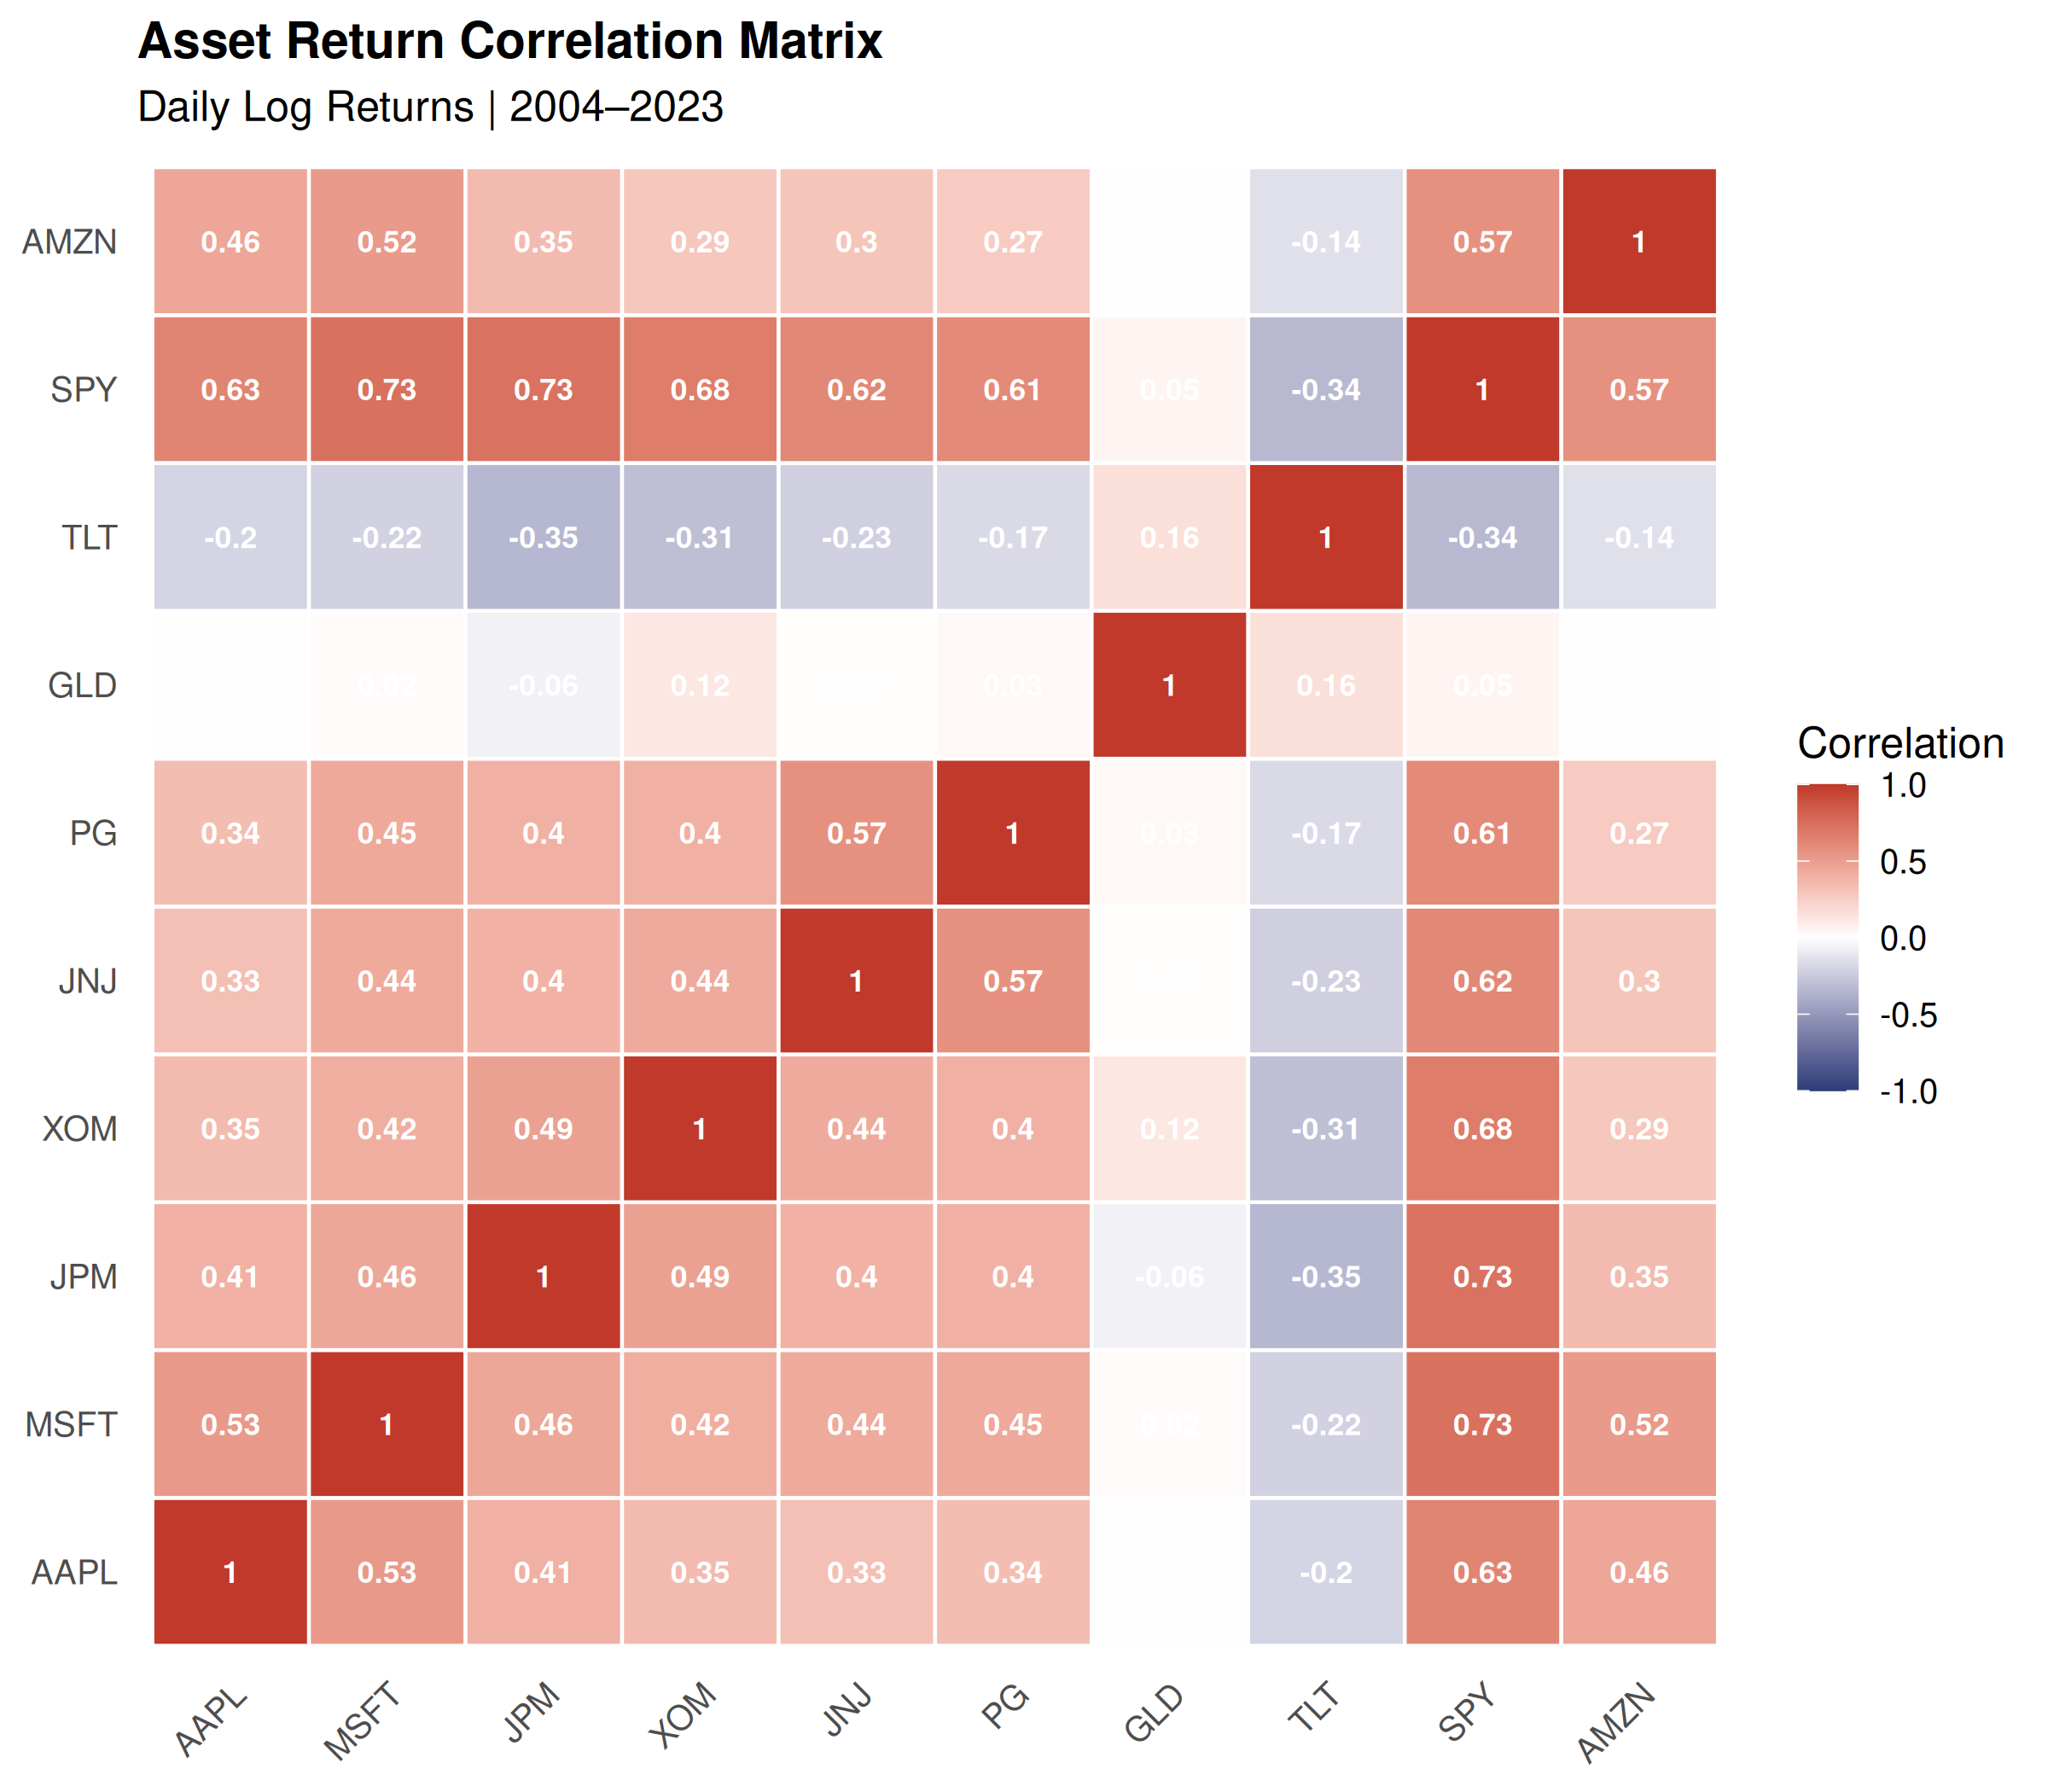
\includegraphics[width=0.85\textwidth]{../outputs/plots/correlation_heatmap.png}
  \caption{Asset return correlation matrix over the full sample period
           (2004--2023). Blue cells indicate negative correlation; red
           indicates positive. TLT and GLD exhibit the strongest
           diversification properties relative to equities.}
  \label{fig:corr}
\end{figure}

\subsection{Frontier Results}

The optimization swept 200 target return levels across the feasible range,
yielding 193 feasible portfolios, of which 173 lie on the efficient upper
half of the frontier. The minimum variance portfolio achieves
$\sigma_{\text{MVP}} = 8.47\%$ and $\mu_{\text{MVP}} = 6.39\%$ annually.

Figure~\ref{fig:frontier} plots the full efficient frontier alongside the
Capital Market Line, individual asset risk-return coordinates, and the
tangency portfolio. The frontier's hyperbolic shape is clearly visible,
with the MVP at its leftmost point. Individual assets lie to the right of
the frontier; none sits on it, confirming that diversification strictly
dominates any single-asset holding in mean-variance space.

\begin{figure}[H]
  \centering
  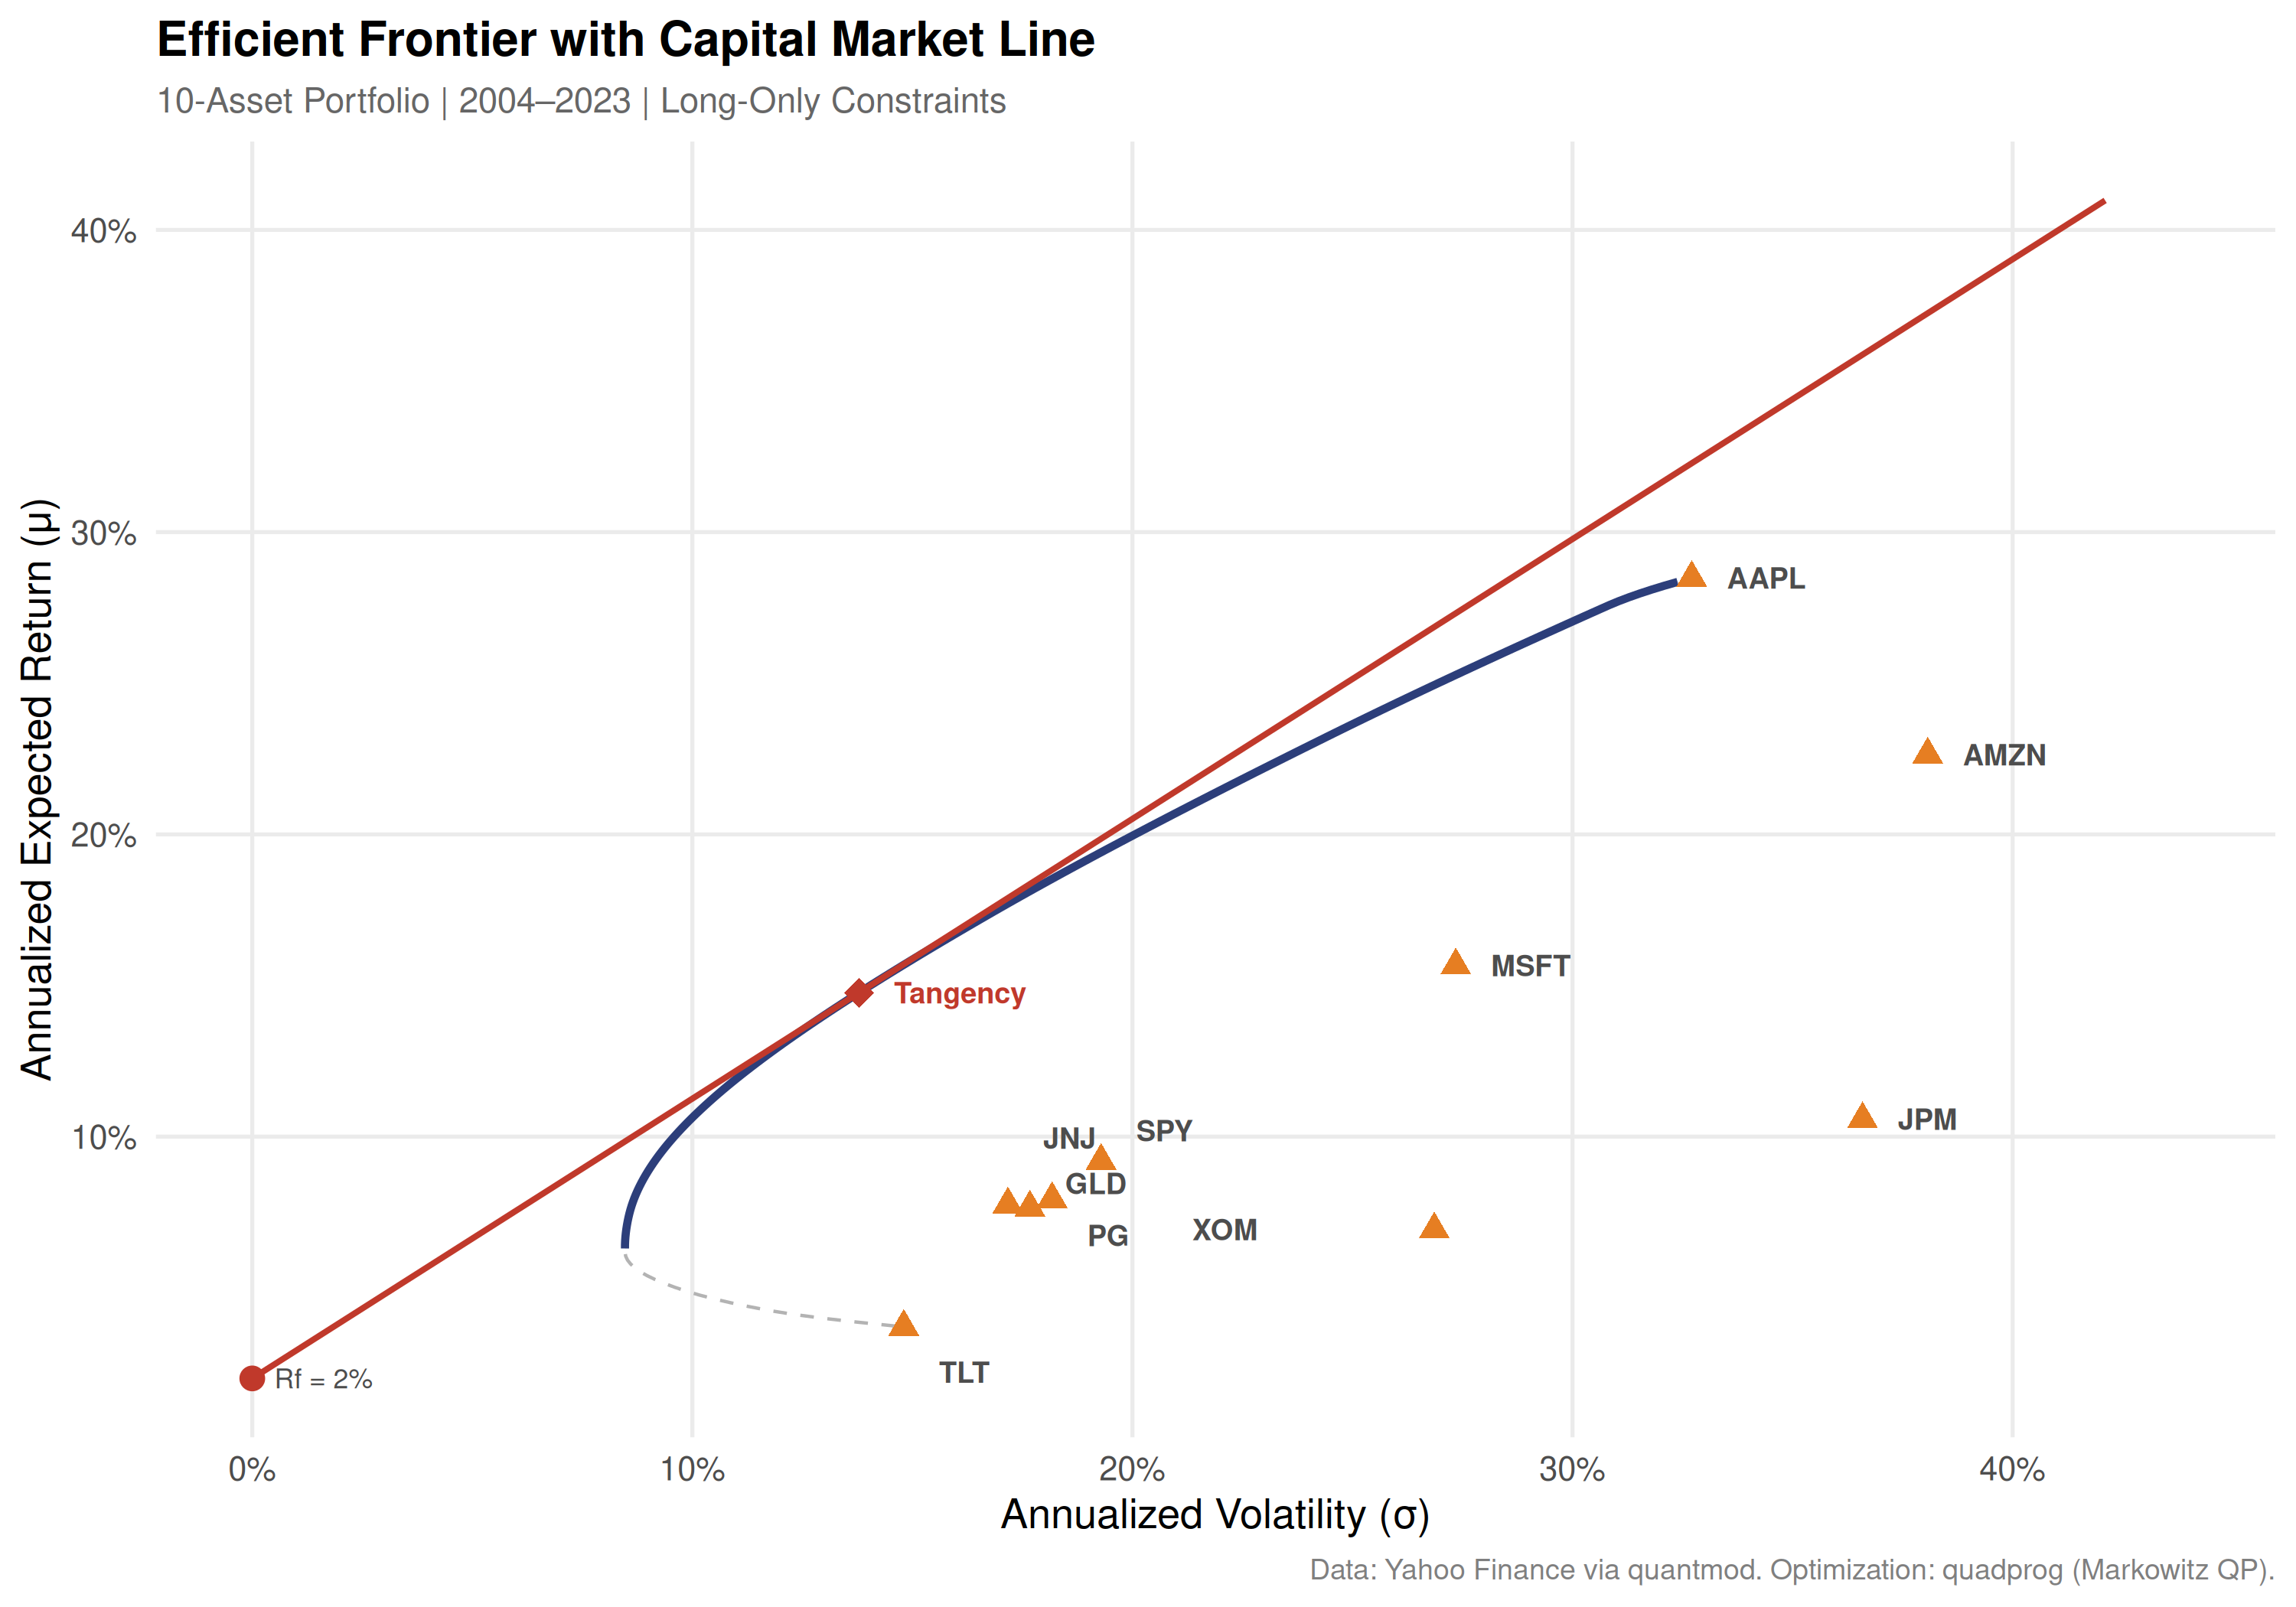
\includegraphics[width=0.88\textwidth]{../outputs/plots/efficient_frontier.png}
  \caption{Efficient frontier, Capital Market Line, and individual asset
           risk-return coordinates. The blue curve is the efficient frontier;
           the dashed grey curve is the inefficient lower half. The red line
           is the CML. Orange triangles are individual assets. The red diamond
           marks the tangency portfolio.}
  \label{fig:frontier}
\end{figure}

% ── Section 5: Capital Market Line and Tangency Portfolio ─────────────────────
\section{Capital Market Line and Tangency Portfolio}
\label{sec:cml}

Assuming a risk-free rate of $r_f = 2\%$, approximating the long-run average
federal funds rate over the sample period, the tangency portfolio achieves:

\begin{equation*}
  \sigma_T = 13.81\%, \quad \mu_T = 14.78\%, \quad
  S_T = \frac{0.1478 - 0.02}{0.1381} \approx 0.926
\end{equation*}

A Sharpe ratio of 0.926 is consistent with long-run equity market performance
and reflects the genuine diversification benefit of combining low-correlation
assets including TLT and GLD with higher-returning equities. The CML passes
cleanly through $(0, 0.02)$ and the tangency point, confirming the geometric
consistency of the optimization.

Under CAPM assumptions, no portfolio above the CML is achievable, and any
portfolio below it is suboptimal; it can be improved by mixing the risk-free
asset and the tangency portfolio. The empirical frontier lies below the CML
everywhere except at the tangency point, as expected.

% ── Section 6: Stress Testing ─────────────────────────────────────────────────
\section{Stress Testing: Crisis Period Analysis}
\label{sec:stress}

\subsection{Frontier Shift Results}

Table~\ref{tab:stress} summarizes the key frontier statistics across all
three estimation periods.

\begin{table}[H]
  \centering
  \caption{Efficient Frontier Statistics Across Periods}
  \label{tab:stress}
  \begin{tabular}{lrrrr}
    \toprule
    Period & MVP $\sigma$ & MVP $\mu$ & Tang. Sharpe & Tang. $\sigma$ \\
    \midrule
    Full Period (2004--2023) &  8.47\% &  6.39\% & 0.926 & 13.81\% \\
    2008 Financial Crisis    & 14.02\% & -1.61\% & 1.029 & 19.52\% \\
    2020 COVID-19 Crash      & 18.33\% & 40.86\% & 2.964 & 22.41\% \\
    \bottomrule
  \end{tabular}
\end{table}

\begin{figure}[H]
  \centering
  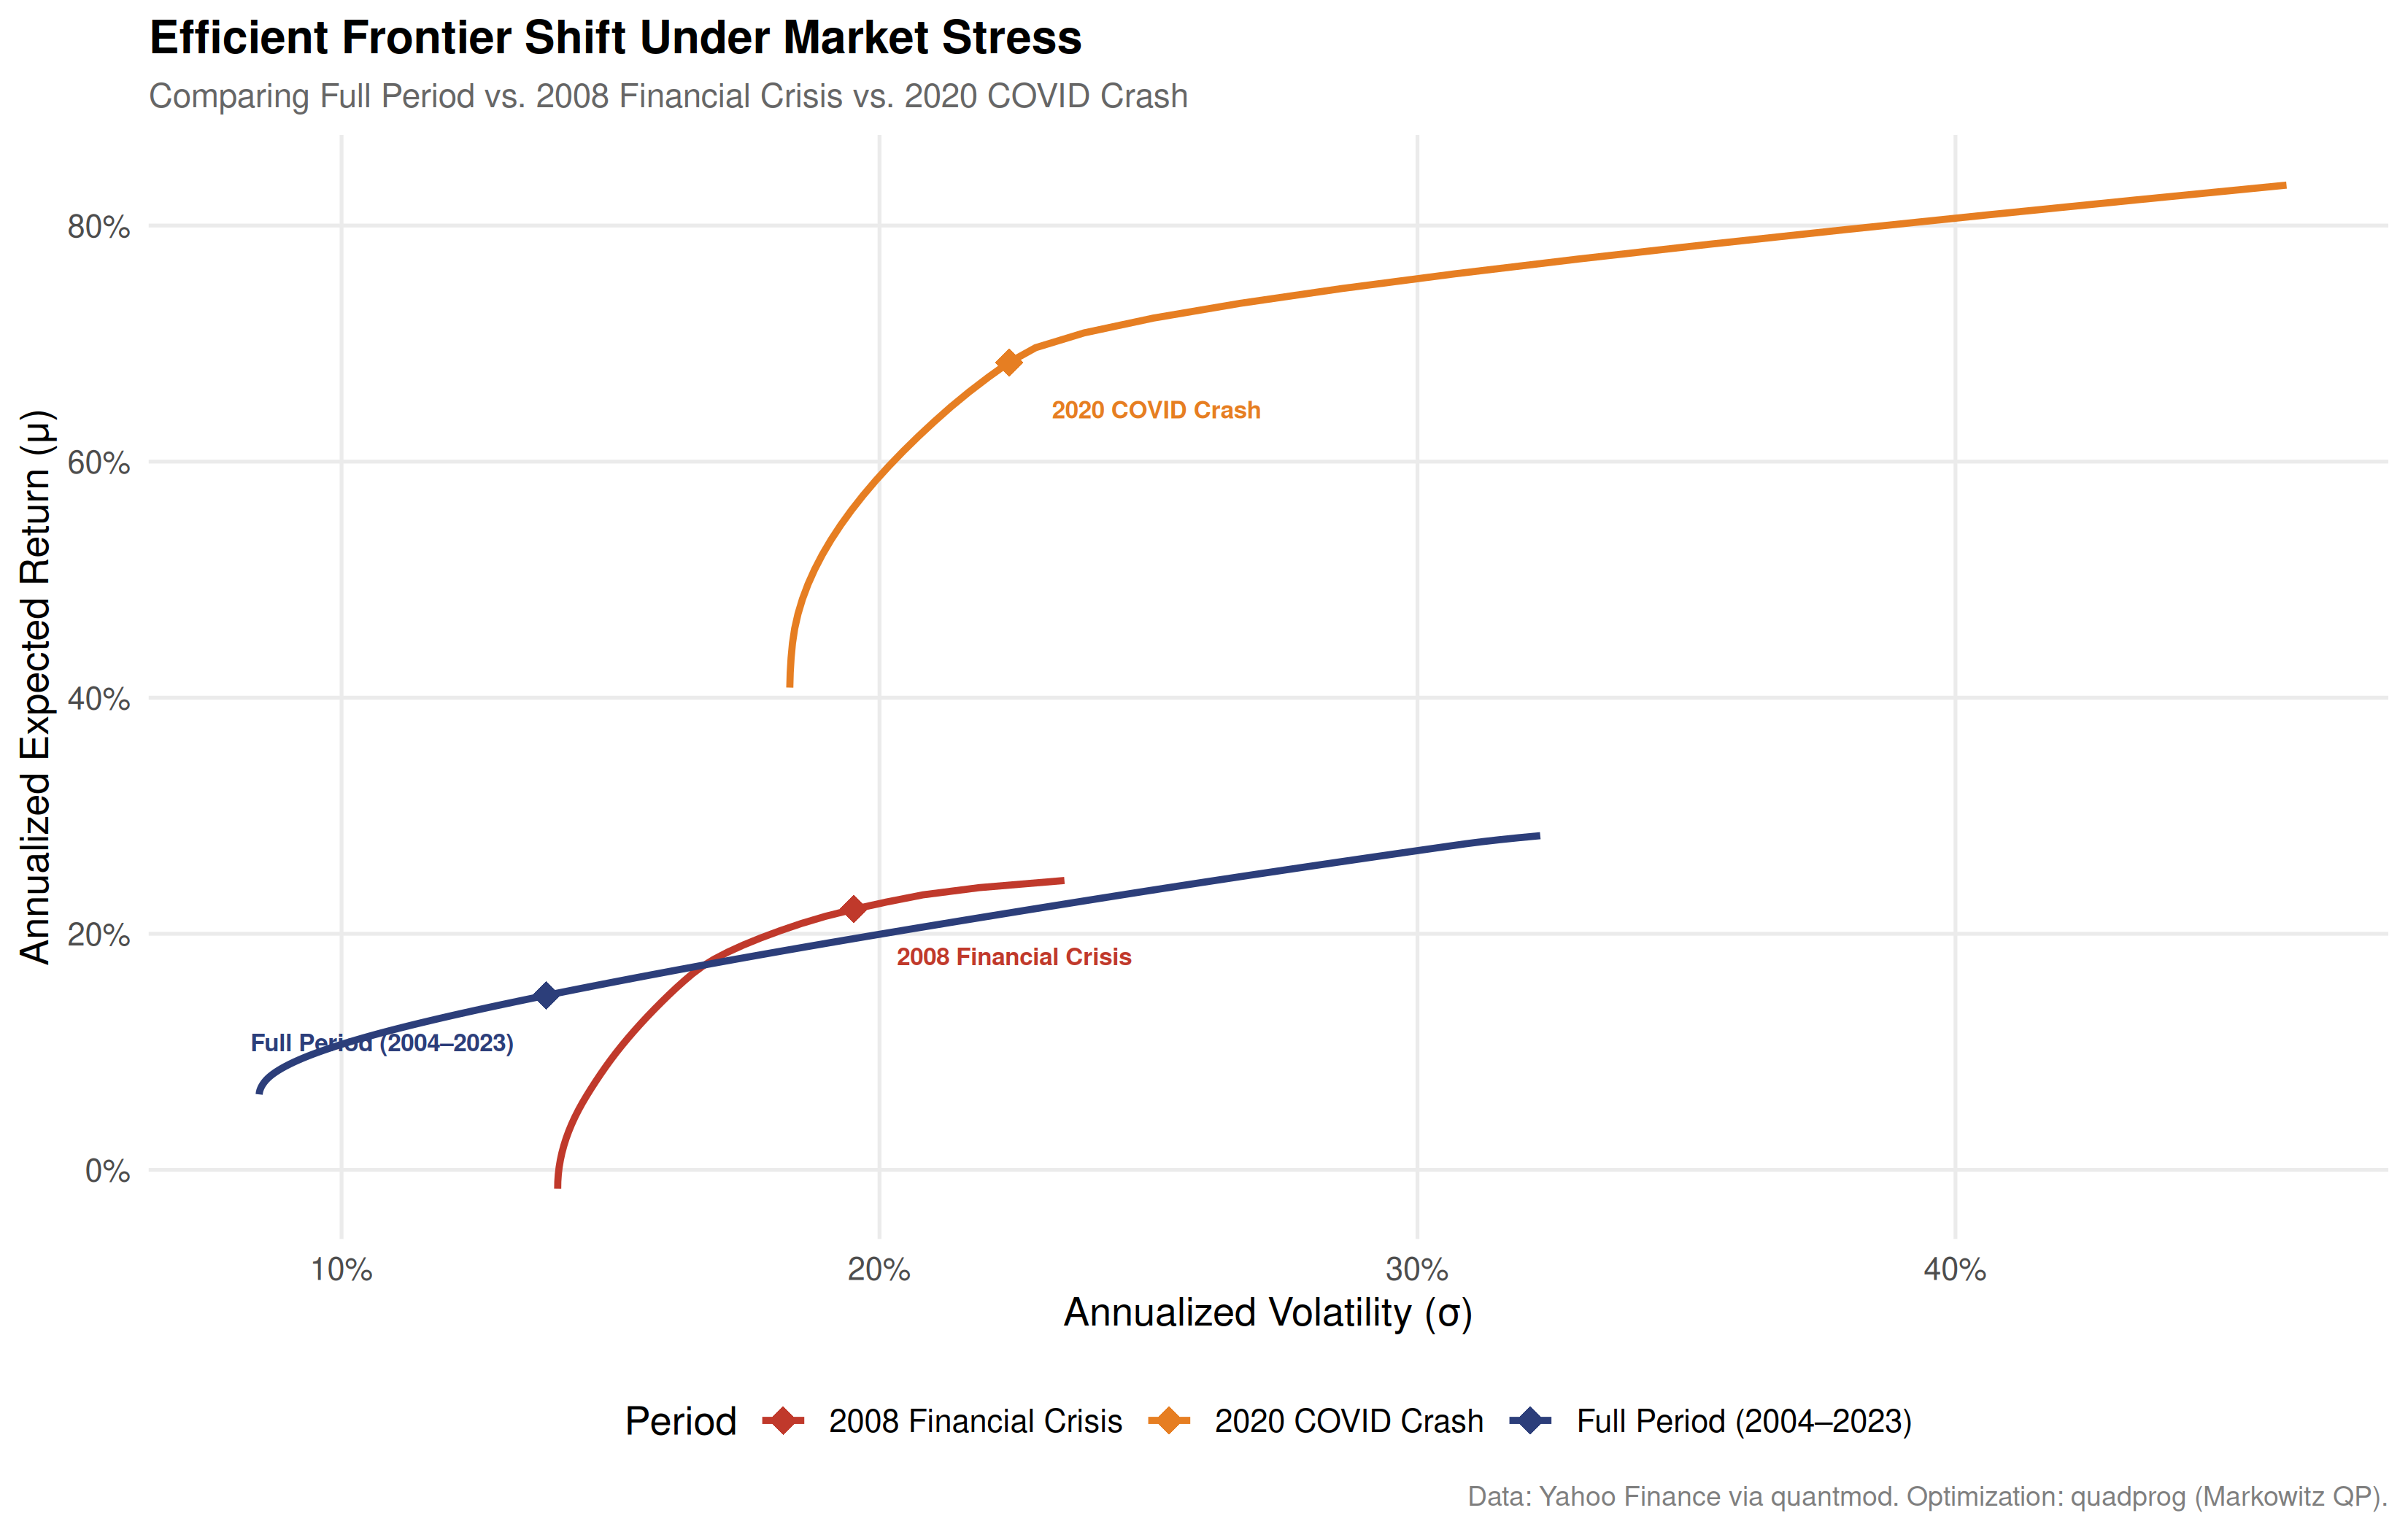
\includegraphics[width=0.88\textwidth]{../outputs/plots/stress_test.png}
  \caption{Efficient frontier shift under market stress. The blue curve
           is the full-period baseline. The red curve is the 2008 crisis
           frontier. The orange curve is the 2020 COVID crash frontier.
           Diamonds mark tangency portfolios for each period.}
  \label{fig:stress}
\end{figure}

\subsection{2008 Financial Crisis}

During the 2008 crisis window, the minimum variance portfolio volatility
increased from 8.47\% to 14.02\%, a 65\% increase in the floor of achievable
risk. Simultaneously, the MVP expected return turned negative at $-1.61\%$
annually. This means the optimizer, even with full freedom to diversify across
all ten assets, could not construct a portfolio with both low risk and positive
expected return during this period.

The mechanism is the correlation breakdown documented extensively in the
crisis literature: during systemic stress, cross-asset correlations spike
toward unity as forced selling and liquidity withdrawal affect all risky
assets simultaneously. The diversification benefit that underpins MVO
evaporates precisely when it is most needed. Our correlation heatmap
(Figure~\ref{fig:corr}), estimated over the full period, masks this dynamic;
a fundamental limitation of static MVO.

\subsection{2020 COVID-19 Crash}

The 2020 results present a different and equally important failure mode.
The optimizer produces a tangency portfolio Sharpe ratio of 2.964 and MVP
returns of 40.86\% annually, numbers that are economically implausible for
a 62-trading-day window during one of the fastest market crashes in history.

This is not a sign that MVO worked better in 2020. It is a sign that the
optimizer overfit severely to a tiny, non-representative sample. With only
62 observations and 10 assets, the sample covariance matrix has condition
number issues and the mean estimates are dominated by noise. The optimizer
finds a portfolio that looks optimal in-sample but would be meaningless
out-of-sample. This is the Michaud (1989) problem in its starkest form:
MVO is, in effect, an error-maximizer when its inputs are imprecise.

% ── Section 7: Limits of MVO ──────────────────────────────────────────────────
\section{The Limits of Mean-Variance Optimization}
\label{sec:limits}

The empirical results of this paper illustrate four structural limitations
of MVO with direct implications for practical portfolio construction.

\textbf{1. Parameter Sensitivity.} MVO is acutely sensitive to the expected
return vector $\boldsymbol{\mu}$. Small changes in return estimates can produce
dramatically different optimal weights, a property that makes the optimizer
unstable in practice. Best and Grauer (1991) showed that a 1\% change in a
single asset's expected return can cause complete portfolio rebalancing. Our
crisis results illustrate this directly: the 62-day 2020 return estimates are
statistically indistinguishable from noise, yet the optimizer treats them as
precise inputs.

\textbf{2. Covariance Non-Stationarity.} The covariance matrix
$\boldsymbol{\Sigma}$ is not a fixed parameter; it is a time-varying stochastic
process. During the 2008 crisis, correlations between equities increased
sharply, causing the frontier to shift rightward and the MVP volatility to
nearly double. Static MVO, which estimates $\boldsymbol{\Sigma}$ from a
historical sample and assumes it forward, cannot capture this dynamic.
Dynamic Conditional Correlation (DCC-GARCH) models address this limitation
but add substantial complexity.

\textbf{3. Non-Gaussian Return Distributions.} Log returns exhibit fat tails,
negative skewness, and excess kurtosis, properties that are particularly
pronounced during crises. MVO's exclusive focus on mean and variance is
theoretically justified only when returns are multivariate normal or
preferences are quadratic. Neither condition holds in practice. Alternative
frameworks such as CVaR optimization or higher-moment portfolio models
explicitly account for tail risk.

\textbf{4. Estimation Window Dependence.} The shape of the efficient frontier
is entirely determined by the estimation window. A 20-year window produces a
stable, well-conditioned frontier. A 3-month crisis window produces an overfit,
economically implausible result. This window-dependence is not a bug in our
implementation; it is a fundamental property of the estimator. Robust
estimation techniques such as shrinkage estimators (Ledoit and Wolf, 2004) or
the Black-Litterman model (1992) partially address this by regularizing the
input estimates.

Despite these limitations, MVO remains foundational. It provides the language,
geometry, and mathematical framework within which virtually all modern portfolio
theory operates. The efficient frontier is not merely a computational output;
it is a benchmark that clarifies what diversification can and cannot achieve,
and under what conditions those achievements hold.

% ── Section 8: Conclusion ─────────────────────────────────────────────────────
\section{Conclusion}
\label{sec:conclusion}

This paper has presented a complete empirical implementation of Markowitz
mean-variance optimization, from raw data ingestion through quadratic
programming to crisis-period stress testing, on a ten-asset diversified
portfolio over the 2004--2023 period. Our results confirm the theoretical
predictions of MVO under stable conditions: the efficient frontier is
well-defined, the tangency portfolio achieves a Sharpe ratio of 0.926, and
diversification demonstrably reduces portfolio risk relative to any individual
asset.

The stress tests reveal the framework's structural limits with precision.
During the 2008 Financial Crisis, the minimum achievable portfolio risk nearly
doubled and the best available expected return turned negative, a direct
consequence of correlation breakdown under systemic stress. During the 2020
COVID crash, the optimizer produced economically implausible results from a
62-day sample, illustrating the error-maximizing property of MVO under
small-sample estimation.

The central lesson is not that MVO is wrong, but that it is conditional. Its
guarantees hold when its assumptions hold: stable covariances, reliable return
estimates, and Gaussian distributions. In practice, these assumptions are most
severely violated during the periods when accurate portfolio optimization
matters most. Practitioners who use MVO without accounting for parameter
uncertainty, covariance dynamics, and tail risk are not applying the framework
incorrectly; they are applying it incompletely.

Future work could extend this analysis by implementing DCC-GARCH to model
time-varying covariances, applying Ledoit-Wolf shrinkage to regularize the
covariance matrix, or replacing variance with CVaR as the risk measure to
better capture tail behavior during crisis periods. Each extension addresses
one of the structural limitations identified here while preserving the core
mean-variance intuition that makes MPT so durable.

% ── References ────────────────────────────────────────────────────────────────
\section*{References}

\begin{enumerate}
  \item Markowitz, H. (1952). Portfolio Selection. \textit{Journal of Finance},
        7(1), 77--91.
  \item Sharpe, W. F. (1964). Capital Asset Prices: A Theory of Market
        Equilibrium Under Conditions of Risk. \textit{Journal of Finance},
        19(3), 425--442.
  \item Black, F., \& Litterman, R. (1992). Global Portfolio Optimization.
        \textit{Financial Analysts Journal}, 48(5), 28--43.
  \item Michaud, R. O. (1989). The Markowitz Optimization Enigma: Is
        Optimized Optimal? \textit{Financial Analysts Journal}, 45(1), 31--42.
  \item Best, M. J., \& Grauer, R. R. (1991). On the Sensitivity of
        Mean-Variance-Efficient Portfolios to Changes in Asset Means.
        \textit{Review of Financial Studies}, 4(2), 315--342.
  \item Ledoit, O., \& Wolf, M. (2004). A Well-Conditioned Estimator for
        Large-Dimensional Covariance Matrices. \textit{Journal of Multivariate
        Analysis}, 88(2), 365--411.
  \item Goldfarb, D., \& Idnani, A. (1983). A Numerically Stable Dual Method
        for Solving Strictly Convex Quadratic Programs. \textit{Mathematical
        Programming}, 27(1), 1--33.
  \item Engle, R. (2002). Dynamic Conditional Correlation: A Simple Class of
        Multivariate Generalized Autoregressive Conditional Heteroskedasticity
        Models. \textit{Journal of Business \& Economic Statistics}, 20(3),
        339--350.
  \item DeMiguel, V., Garlappi, L., \& Uppal, R. (2009). Optimal Versus
        Naive Diversification: How Inefficient is the 1/N Portfolio Strategy?
        \textit{Review of Financial Studies}, 22(5), 1915--1953.
  \item Rockafellar, R. T., \& Uryasev, S. (2000). Optimization of
        Conditional Value-at-Risk. \textit{Journal of Risk}, 2(3), 21--41.
\end{enumerate}

\end{document}